\clearpage

\documentclass[oneside,a4paper,titlepage]{article}
\usepackage{blindtext}
\usepackage[utf8]{inputenc}
\usepackage{pdfpages}
\usepackage{graphicx}
\usepackage{geometry}
\usepackage{float}


\begin{document}

\section{Beskrivelse - Hvordan forløb processen i P1}
% I skal beskrive jeres P1 projektproces så detaljeret som muligt. I må gerne komme ind på alle de aspekter I finder relevante. I skal komme ind på følgende områder:

Lige efter gruppedannelsen skete der ikke så meget i projektet, da vi var meget i tvivl om vores projektforslag. Projektforslaget var ikke fremstillet på samme måde som de andre. Under et af lektionerne til PV skulle vi i gruppen udfylde en række spørgsmål til  hvordan gruppen f.eks.\ ville håndtere konflikter og hvordan vores samarbejdsaftale så ud. Disse spørgsmål kan ses i bilag \ref{sec:samarbejdsaftale}. Der var også en lektion i PV, der handlede om at få styr på projektet, denne omhandler planlægning, værktøjer og roller \ref{sec:styr_paa_projektet}.\newline\newline
I gruppen benyttede vi os meget af "Peer-learning". Grunden til dette var, at gruppens medlemmer havde forskellige kompetencer og dette kunne vi udnytte vi at hjælpe hinanden. Vi hjalp hinanden ved at et gruppemedlem lavede en kort fremlæggelse på tavlen, så de andre gruppemedlemmer, om ikke andet, kunne få en nogenlunde forståelse og et godt udgangspunkt til viderearbejde.
Til konflikter som f.eks.\ overskredede deadlines eller at komme for sent til gruppearbejde har vi været meget tolerante. Enten er deadlines blevet rykket eller man har givet kage hvis man er kommet meget for sent i en længere periode. \newline\newline
Til disse spørgsmål havde vi til samarbejdsaftalen aftalt at møde 8:15 og derefter arbejde fra 8:30 til 16:15. Efterhånden som projektet forløb blev dette lavet om til at møde 8:30 og derefter til vi ikke rigtigt gad mere og havde nået det vi ville på dagen. Vi har ikke udarbejdet en fast tidsplan, men der er derimod en konsensus om, at der er frokost klokken 12. Der er dage hvor frokosten rykker sig, hvis vi glemmer tiden når vi har været meget fokuseret på arbejdet. Vores skriftlige samarbejdsaftale er derfor ikke særlig lang, vi har dog mange mundtlige aftaler og gensidig respekt for hinanden. \newline\newline
Vi lavede en Belbin rolletest, hvor vi på baggrund af denne, bestemte gruppens kontaktperson og hvem der skulle træde til som leder, hvis det blev nødvendigt. Vi har derfor ikke haft en fast projektleder, da vi mente det var unødvendigt og formentlig fordi vi på daværende tidspunkt syntes det ville være lidt akavet at skulle agere chef over for de andre i gruppen.\newline\newline
Til samarbejde med vores vejledere, gav begge vejledere os en liste over hvilke krav de havde til samarbejdet. Disse lister har fungeret som vores samarbejdsaftale med vejlederne. De omhandlede bl.a.\ i hvilket format arbejdsblade skulle sendes i, hvor lang tid de skulle have til at læse dem og at kun referentens computer skulle være åben til vejledermøderne. Inden et vejledermøde havde vi lavet en agenda, som på forhånd blev sendt til vejlederen. Vi havde to former for vejledermøder: Den ene var at vi sendte vores arbejdsblade hvorefter vi vil få feedback i form af kommentarer over mail. Den anden var det mere traditionelle vejledermøde hvor vejlederen havde udprintet rapporten og kommentarerne blev diskuteret ansigt til ansigt. \newline\newline
Da vi skulle til at lave den initierende problemstilling lavede vi en overordnet tidsplan til hvornår vi skulle have de store emner gjort færdigt. Ud fra denne sørgede vi at give os selv opgaver og deadlines løbende, så disse mål ville blive opfyldt. \newline
Når vi skulle uddele opgaver til os selv, havde vi skrevet opgaverne op og derefter kunne man selv sætte sig på noget eller blive sat på noget af en anden person, efter aftale. Motivering i gruppen kom løbende, vi motiverede hinanden og hjalp til, så vi ikke kørte død i skrivearbejdet. Jokes, små spil og sociale pauser hjalp meget med dette. 
Hver morgen lavede vi dagsordener til hvad vi vil lave den dag. Dette hjalp med at overholde tidsplanen. Til at organisere vores arbejde har gruppen benyttet sig af Trello \ref{trellolink}, da det er meget nemt at lave nye kort med opgaver og man kan hurtigt få oversigt over dem. Som det kan ses på figur \ref{fig:trello} kan man se hvem der er på hvilke opgaver og hvor langt opgaven er fra at være færdig.

\begin{figure}[H]
    \centering
    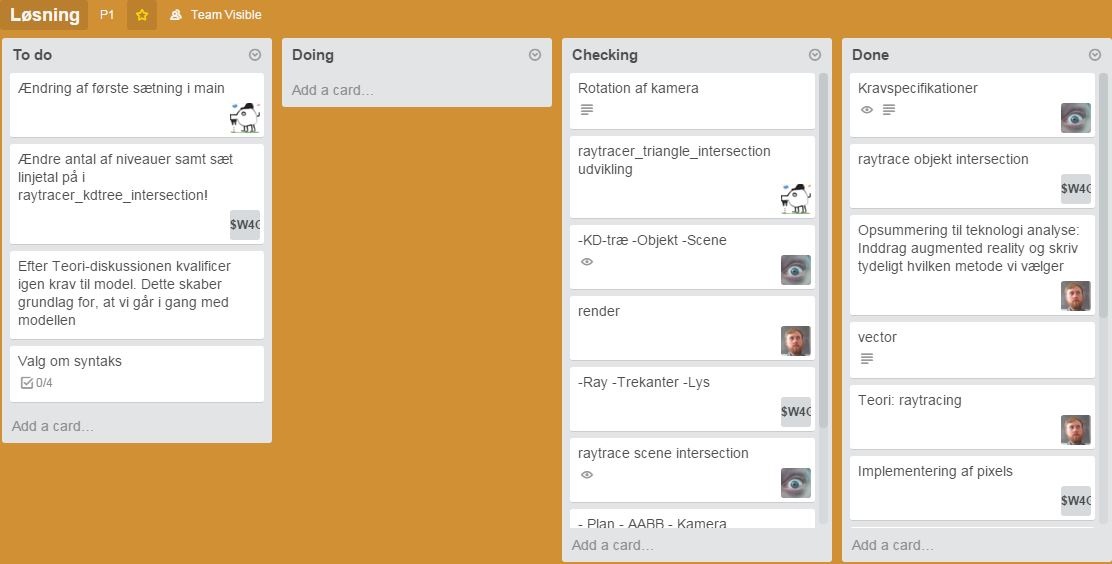
\includegraphics[width=15cm]{./../graphics/trello}
    \caption{Et udklip fra vores løsningsboard på Trello}
    \label{fig:trello}
\end{figure} 
Vi brugte Git til vores version-control således at alle hurtigt kunne den hente den nyeste version. Git blev også brugt til at holde styr på koden. I forbindelse med projektet kontaktede vi flere personer og virksomheder, vi skrev til 10 lampebutikker, to designere og IKEA. Ansvar for denne kommunikation lå på kontaktpersonen, som var ansigtet ud ad til. \newline\newline
Opgaverne uddeltes for de meste med først-til-mølle-princippet, men der blev stadigt taget højde for omfanget af opgaven, så det ikke endte med at en person havde en 30 minutters opgave mens en anden havde en to timers opgave. Enten ville personen med den lille opgave få noget mere at lave ellers ville personen med den store opgave opdeles og laves af flere. Vi holdte korte og uformelle møder her og der, hvor vi kom med en status på mangler og lignende i rapporten eller koden. Da møderne i sig selv var så uformelle, var der ingen mødeleder eller runde om bordet. Hvis man havde noget at byde ind med bød man ind. \newline\newline
Vi havde ikke haft en seriøs snak om hvad vi forventede af hinanden, det lå meget implicit da vi arbejdede. Der var dog nogle forventninger, der var blevet sagt f.eks.\ at vi mødte til tiden og at man lavede det man blev bedt om. Ambitionen lå selvfølgelig højt, vi ville gerne lave noget vi kunne stå inde for og gøre vores bedste. Vi forventede ikke at gruppemedlemmer tog med på bar eller andet, hvis de ikke har lyst. Det var noget man selv bestemte om man ville eller ej, vi ville dog stadig spørge efter det og prøve at få en person til komme med, da vi kun havde kendt hinanden i under et halvt år. \newline\newline
Vi hjalp hinanden med gruppeopgaver til det forskellige kurser. I programmering foregik dette ved at vi fælles skrev koden og viste den på en projektor. I matematik lavede vi opgaver selv så meget som muligt, men man kunne frit slå sig sammen med en anden eller spørge. Vi sørgede for at alle havde en forståelse for hvordan opgaven skulle løses. Hvis én forstod noget som nogle andre ikke gjorde holdte denne person ofte en kort fremlæggelse på tavlen, så de andre havde en god nok forståelse til at kunne lave opgaverne. \newline\newline
En af de arbejdsprocesser som vi havde i gruppen, var at vi hver morgen lavede en dagsorden for dagen. Vi vil i dette afsnit kort forklare og illustrere nogle af de dagsplaner som vi havde under P1. 
Her er et par eksempler på dagsordner i løbet af projektet:
\paragraph{Dagsorden 9/10/15:}
\begin{itemize}
  \item Brainstorm.
  \item Diskussion af spørgsmål til styringsgruppe mødet.
  \item Agenda.
  \item Find de programmer vi vil bruge til projektarbejde, heraf undersøg Trello, og Github.
  \item Opsummering og afrunding  af dagen.
\end{itemize}
Her ses en typisk dagsorden for starten af projektet, hvor vi brugte lang tid på at diskutere hvilket emne vi ville arbejde med, samt at få styr på praktiske ting som programmer til fildeling.
Et andet eksempel på en dagsorden kunne se således ud:
\paragraph{Dagsorden 20/11/15:}
\begin{itemize}
  \item Agenda til Annette.
  \item Planlæg.
\end{itemize}
I slutningen af projektet var der fokus på at samle trådene og en dagsorden så derfor ofte således ud:

\paragraph{Dagsorden 14/12/15:}
\begin{itemize}
  \item Revidere afgrænsning af løsningsforslag.
  \item Skrive afsnit om rotationsmatricer i udviklingsafsnittet.
  \item Fordele og ulemper ved augmented reality.
  \item Skitse til Phong.
  \item Ret sekvensdiagram.
  \item Skriv testafsnit færdigt.
\end{itemize}
Her ses der en dagsorden lavet nogle dage før projektafleveringen, og her er der fokus på at rette eventuelle mangler.

%læreprocessen (herunder problemorienteringens røde tråd)

%Det er vigtigt at I venter med at analysere jeres erfaringer til efter at I er færdige med at beskrive dem ! 

\section{Vurdering - Hvordan gik det}
\begin{itemize}
  \item Opgaveuddeling ved hjælp af Trello gik godt i starten og knap så godt i slutningen af projektet.
  \item Git som version-control var rigtigt god til at holde styr på koden, men knap så god til latex.
  \item Dagsordenerne gik godt, men nogle gange var de meget korte og upræcise.
  \item Grupperolletesten er slet ikke blevet brugt udover at give os selv kendskab til hvilke roller vi har.
  \item Vejledersamarbejdet gik godt.
  \item Samarbejdet med erhvervslivet hjalp meget med god viden til viden rapporten, selvom vi blev afvist af IKEA.
  \item Kommunikationen i gruppen er hovedsageligt god og samtaler kan godt afsluttes når vi skal arbejde. 
  \item Nogle i gruppen kan være ufokuseret og følger ikke med om morgenen når dagsordenen laves, hvilket ofte ender i at den person ikke laver noget.
  \item Gruppens konflikthåndtering har været meget dårlig.
  \item Vi har været dårlige til at stå op og "skælde" en person ud hvis de ikke følger med.
  \item Gennemgang af rettelser på projekter var godt.
  \item Fællesregning af gruppeopgaver fra kurser var godt.
  \item Gruppesamarbejdet gik okay, der var nogle gode ting og nogle dårlige ting. 
\end{itemize}
%Hvordan er kommunikationen i jeres gruppe ? Er der nogle der taler hele tiden ? Er der nogen der aldrig siger noget ? Bruger gruppen uforholdsvis lang tid på diskussionerne ? Hvorfor ?
\section{Analyse – Hvorfor gik det som det gik?}
Opgavefordelingen gik lidt i stå hen mod slutningen af projektet da det blev meget uoverskueligt og vi synes du var lettere at skrive det vi skulle lave op på tavlen. Vi glemte ofte at flytte kortene til hvor du skulle være. Nogle gange kunne det føles som ekstra arbejde at skulle ind og flytte et kort når man gik igang og igen når man var færdig. \newline\newline
Git fungerede rigtig godt fordi et par stykker i gruppen havde kendskab til det og hjalp de andre i gang så alle kunne bruge det nogenlunde selvstændigt. Vi fik dog mange mergefejl når vi skrev i latex, da der ofte blev skrevet i de samme dokumenter. Git var dog rigtig god til at holde styr på koden, da der ofte ikke var lige så meget aktivitet og koden var delt op efter top-down metoden, hvilket medførte at vi nærmest aldrig skrev i den samme fil. \newline\newline
Dagsordenerne blev nogle gange meget korte og upræcise, dette kan være fordi at ikke alle i gruppen var med til at skrive dem. 
Grupperolletesten vidste os hvilke roller vi havde, som nogle vidste i forvejen fra gymnasiet. Den hjalp med at finde ud af gruppens styrker og svagheder, selvom det ikke blev benyttet meget. 
Vejledersamarbejdet gik godt fordi vores vejledere virkede meget engagerede i emnet og kom med god feedback og svarede hurtigt når der blev spurgt om noget. Det hjalp også meget at de stillede krav til hvordan de ville samarbejde med os. 
Samarbejdet med erhvervslivet gik godt fordi vi fik kontakt til at del personer, der arbejder med lamper til hverdag og var villige til at svare på spørgsmål fra os. Desværre måtte vi ikke uddele det spørgeskema i IKEA vi havde lavet, da butikschefen i Aalborg mente at vi satte IKEA i et dårligt lys ved at spørge deres kunder om utilfredshed. \newline\newline
Kommunikationen i gruppen var god, da vi alle er unge og har nogle fælles interesser. Nogle i gruppen kendte også hinanden fra tidligere grupper, hvilket også hjalp.
Da vi alle bor forskellige steder møder vi ikke på samme tid. Nogle, der kommer tidligt ind kan begynde at lave noget som ikke er studierelevant, mens der ventes på de andre. Det kan dog ofte være svært at få afsluttet det man er igang med, så derfor vil personen ikke følge særligt meget med i starten. 
Vi har ikke haft nogle seriøse konflikter, som at smide nogle ud af gruppen. Vi har dog været dårlige til at få sagt at folk skal høre efter når vi laver noget fælles. Det eneste der har været lidt træls er at et gruppemedlem valgte at droppe ud så vi næsten ikke kunne nå at indberette det til studiesekretæren inden deadline. \newline\newline
Vi har haft adgang til en projektor i grupperummet, som har hjulpet meget når vi skal lave fælles arbejde, da vi alle kan sidde på vores egen plads og følge med på skærmen. Den var især nyttig når vi skulle gå igennem rettelser til rapporten fælles og afprøve ændringer. Den blev også brugt til at lave gruppeopgaver i programmering. Når vi skulle lave opgaver i matematik satte vi os også sammen og lavede dem nogenlunde fælles, og hvis noget ikke kunne forstås blev dette forklaret hvilket hjalp meget. 

%Dernæst skal I analysere jeres arbejdsprocesser og få klarlagt hvorfor noget gik godt mens andet gik dårligt. Med andre ord: Hvad er det for faktorer, som har indvirket på arbejdsprocesserne? 

\section{Syntese – Gode råd til P2}
% samarbejdsaftale, snakke sammen om konflikter og engagement
Vi vil her lave en såkaldt "start-stop-fortsæt" liste om hvad vi vil starte med at gøre i P2, som vi ikke gjorde i P1. Hvad vi ikke vil gøre i P2, som vi gjorde i P1 og hvad vi vil fortsætte med at gøre i P2, som vi også gjorde i P1.
%Hvis jeres vurdering og analyse skal bidrage til at forbedre jeres evne til at håndtere det problemorienterede og projektorganiserede gruppearbejde, skal I til slut konkretisere jeres erfaringer i nogle ’Gode råd’ til jer selv og jeres medstuderende. En god måde at formulere sådanne gode råd på er som en *start-stop-fortsæt*-liste, dvs. en liste med følgende tre sektioner:
%– Dette vil vi begynde at gøre i P2, som vi ikke gjorde i P1 
%– Dette vil vi ikke gøre i P2, som vi gjorde i P1
%– Dette vil vi fortsætte med at gøre (gerne anderledes og bedre) i P2, som vi også gjorde i P1 
\paragraph{Start}
\begin{itemize}
  \item Vi vil overveje at bruge ShareLatex til rapporten. 
  \item Vi vil bruge en dag i starten af projektet til at diskutere arbejdsindsats og hjemmearbejde. 
  \item Vi vil starte med at lægge alt elektronisk udstyr væk så længe vi laver fælles ting i gruppen (opgaver, diskutioner mm.).
  \item Vi vil lave en mere udførlig samarbejdsaftale, som kan hjælpe med konflikter og kan give konsekvenser. 
  \item Vi vil starte med at organisere sociale events for at styrke gruppen samvær og gøre os mere trygge ved hinanden.
  \item Vi vil starte med at bruge funktionen \textbackslash autoref til latex, i stedet for \textbackslash ref da \textbackslash autoref automatisk kan skrive afsnit foran, hvilket vil hjælpe på konsistens og sådanne fejl kan være svære selv at finde.
\end{itemize}

\paragraph{Stop}
\begin{itemize}
  \item Vi vil stoppe med at bruge Trello til alt, og derved formindske mængden af kort så det bliver mere overskueligt.
  \item Vi vil stoppe med at bruge alt for lang tid på at diskutere i gruppen, selvom det er relevant for projektet. Årsagen til dette er, at tiden hurtigt kan forsvinde og ikke alle i gruppen vil blive i grupperummet efter 16:15.
\end{itemize}

\paragraph{Fortsæt}
\begin{itemize}
  \item Vi vil fortsætte mig at bruge Git til versioncontrol af vores kode.
  \item Vi vil forstætte med at lave dagsordner hver dag vi møder i grupperummet.
  \item Vi vil fortsætte med at have en projekter eller lignende i grupperummet, både til at gennemgå rettelser til rapporten og fælles arbejde til kurser. 
  \item Vi vil fortsætte at uddele opgaver på tavlen når vi arbejder i grupperummet og krydse af når de er lavet. Dette begyndte vi først på den sidste uge, men det gav et godt overblik over de enkelte opgaver der skulle laves inden aflevering.
  \item Vi vil forstætte med at lave en overordnet tidplan tidligt, for at give os selv realiske mål for hvad vi kan og skal nå.
  \item Vi vil fortsætte med at rette stavefejl og andre småting løbende, da det hjælper meget på presset i dagene op til aflevering. 
  \item Vi vil fortsætte med at lave en tidlig struktur til rapporten, da det gør det lettere at uddele opgaver og sørger for at vi holder den røde tråd så meget som muligt. 
  \item Vi vil fortsætte med at lave en agenda og tage referat til vejledermøder.
  \item Vi vil fortsætte med at have en facebooksamtale, hvor vi kan være sociale men også spørger efter projektrelevante ting når vi laver hjemmearbejde.
  \item Vi vil fortsætte med at holde små fremlæggelser for hinanden, hvis det er nødvendigt at noget bliver forklaret enten til projektet eller til kurserne, hvor bøgerne kan være lidt kryptiske. 
  
\end{itemize}
%Spørgsmål til inspiration
%Projektplanlægning
%Har alle i gruppen samme opfattelse af hvad projektplanlægning er ? Find ud af det.
%Hvad vil I foreslå til planlægning og styring af et P2 projekt ?

%Samarbejdet i gruppen
%Hvilke forventninger har I til samarbejdet i P2 ? Hvordan skal de blive opfyldt ?

%Samarbejdet med vejlederne
%Hvilke forventninger vil I stille til jeres vejledere i P2 ?

%Læreprocesserne
%Hvordan lærer du bedst ?
%Hvordan har I brugt resultaterne af jeres individuelle læringstest ?
%Hvordan hjælper/stimulerer vejlederen jeres læreprocesser ?
%Hvilken læringsstrategi er bedst til kurser ?
%Hvilken læringsstrategi er bedst til projektarbejde ?

\clearpage
\section{Bilag}
\subsection{Belbins teamroller}
\label{sec:styr_paa_projektet}
\section*{PV – Få styr på projektet}
\subsection*{Planlægning}
\begin{itemize}
  \item Initierende problem – 15 / 10
  \item Problemanalyse \& problemformulering – 14 / 11
  \item Løsning (metode) – 14 / 11
  \item Udvikling – 7 / 12
  \item Dokumentation – 12 / 12
  \item Konklusion – 14 / 12
  \item Afslutning og aflevering – 18 / 12
  \item Procesanalyse – 22 / 12
\end{itemize}

\subsection*{Værktøjer}
\begin{itemize}
  \item Trello
  \item Github
  \item Latex
  \item Google docs
\end{itemize}
Trello er til opgaveadministration.
Git er til version-control.
Docs er til fællesrettelser.
Latex er det system vi skriver rapporten i.
\subsection*{Roller}
\begin{itemize}
  \item Kontaktperson: Lasse
  \item Referent: Skiftende rolle
  \item Ordstyrer: Skiftende rolle
  \item Leder: Anton og Morten
\end{itemize}
Gruppen har taget en rollemodels test: \newline
Kristian Træhold: Formidler og Specialist. \newline
Christian Grunberg: Formidler og Organisator.\newline
Mathias Ibsen: Formidler og Specialist.\newline
Lasse Gadegaard: Organisator, kontaktskaber og formidler.\newline
Mathias Pihl: Organisator og specialist.\newline
Morten Rask: Organisator, koordinator, opstarter, afslutter, specialist.\newline
Anton Christensen: Koordinator, opstarter.\newline

\subsection*{Rollebeskrivelser}
Formidler: Social personlighed som er meget diplomatisk og løser konflikter.
Specialist: Har en stor faglig viden indenfor et område. Fokuserer på sit arbejde.
Organisator: Sørger for at tingene er i orden, og at vi har en tidsplan.
Kontaktskaber: Social person der holder styr på kommunikation, og alt det formelle.
Koordinator: Leder som tager beslutninger, og uddelegerer opgaver
Opstarter: Er god til at sætte folk i gang, og vil hele tiden lave noget
Afslutter: En der kan samle trådene, og ikke lader et projekt løbe ud af tangenter
Idémand: En person som altid ser nye muligheder og er en god debatstarter.

\begin{figure}[H]
   \centering
   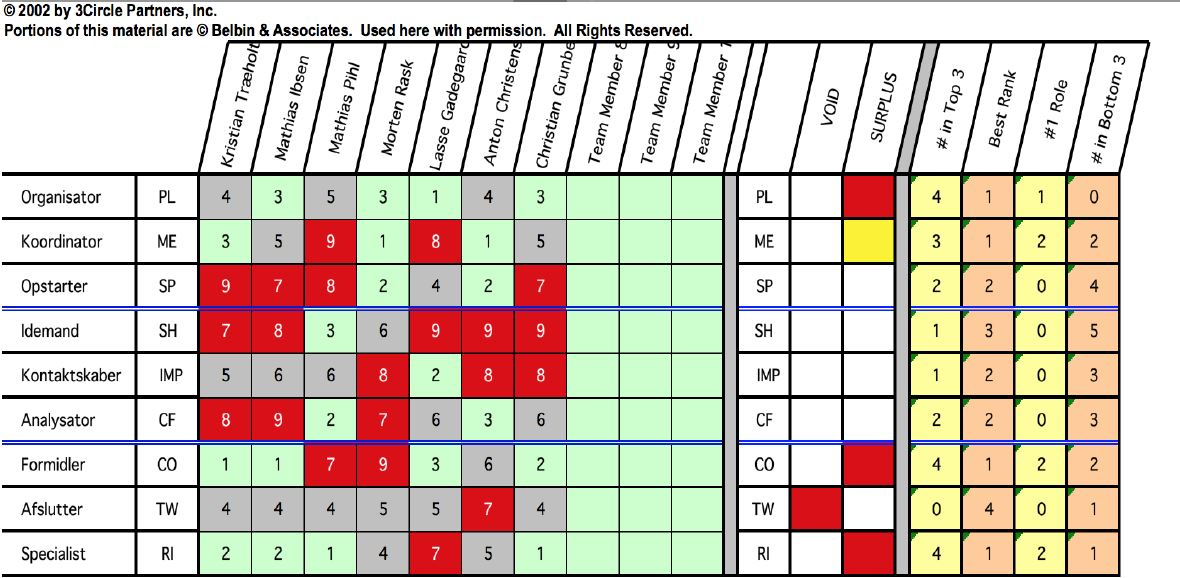
\includegraphics[width=15cm]{./../graphics/rolletest}
   \caption{Resultatet af rolletesten}.
\end{figure}

\subsection*{Kommentar til skema:}
Vi kan se, at der generelt er en fin fordeling af roller, hvor den eneste, som ikke er grøn er ”afslutter”, men her ses der at mange gruppemedlemmer har denne som 4 og 5 prioritet. Det er derfor oplagt at tage denne i fællesskab. Derudover har vi 3 roller der er i SURPLUS. Her skal vi være opmærksom på, at der ikke bliver lavet for meget dobbeltarbejde, og at vi alle går i samme retning.

\subsection{Samarbejdsaftale mm.}
\label{sec:samarbejdsaftale}

\section*{Hvordan benytter gruppen resultaterne fra læringsstiltestene til at gruppemedlemmerne lærer bedre ”til og fra hinanden” (Peer læring)?}
Vi har fået en forståelse for at folk lærer og opfatter tingene på forskellige måder. Vi skal derfor være åbne for forskellige forslag, og have en accept for at folk lærer på forskelligt. Derudover skal vi inkorporere de forskellige læringsmetoder i vores gruppearbejde, hvor personer der f.eks. lærer bedst ved ”forklaring” – også får en mulighed for at forklare hvad personen har lært for andre.
\section*{Hvad vil i gøre i gruppen, hvis der opstår konflikter, som kræver en løsning?}
Vi skal finde frem til kernen af konflikten. Vi diskuterer efterfølgende problemet, hvor vi har en ordstyrer som styrer slagets gang, og alle får derefter lov til at udtrykke deres meninger og holdninger til problemet. Derefter kan man finde eventuelle ligheder og forskelle, og derudfra finde en løsning på konflikten.
\section*{Hvordan ser gruppens samarbejdskontrakt ud?}
Vi møder hverdag kl 8:15 og begynder gruppearbejdet 8:30. Hvilket vil sige, at man har 15min til ”fri leg” og sociale samtaler.
Normal arbejdsdag: 8:30 – 16:15 med mulighed for ændringer hvis ALLE er enige.
Vi vil lave et mål for hver dag. Altså en dagsorden for hvad der skal nås.
Man SKAL informere ”inden” mødetid hvis man ikke kan møde til tiden.
\section*{Vejleder:}
At vi foreslår, at vores arbejdspapirer bliver delt over Google Docs. og vejlederen har derefter mulighed for at kommentere i Google Docs. Vi laver en redigeringsaftale med vejlederen.
Lav en Agenda til hver møde.

\clearpage
\subsection{Brainstorm}
\begin{figure}[H]
   \centering
   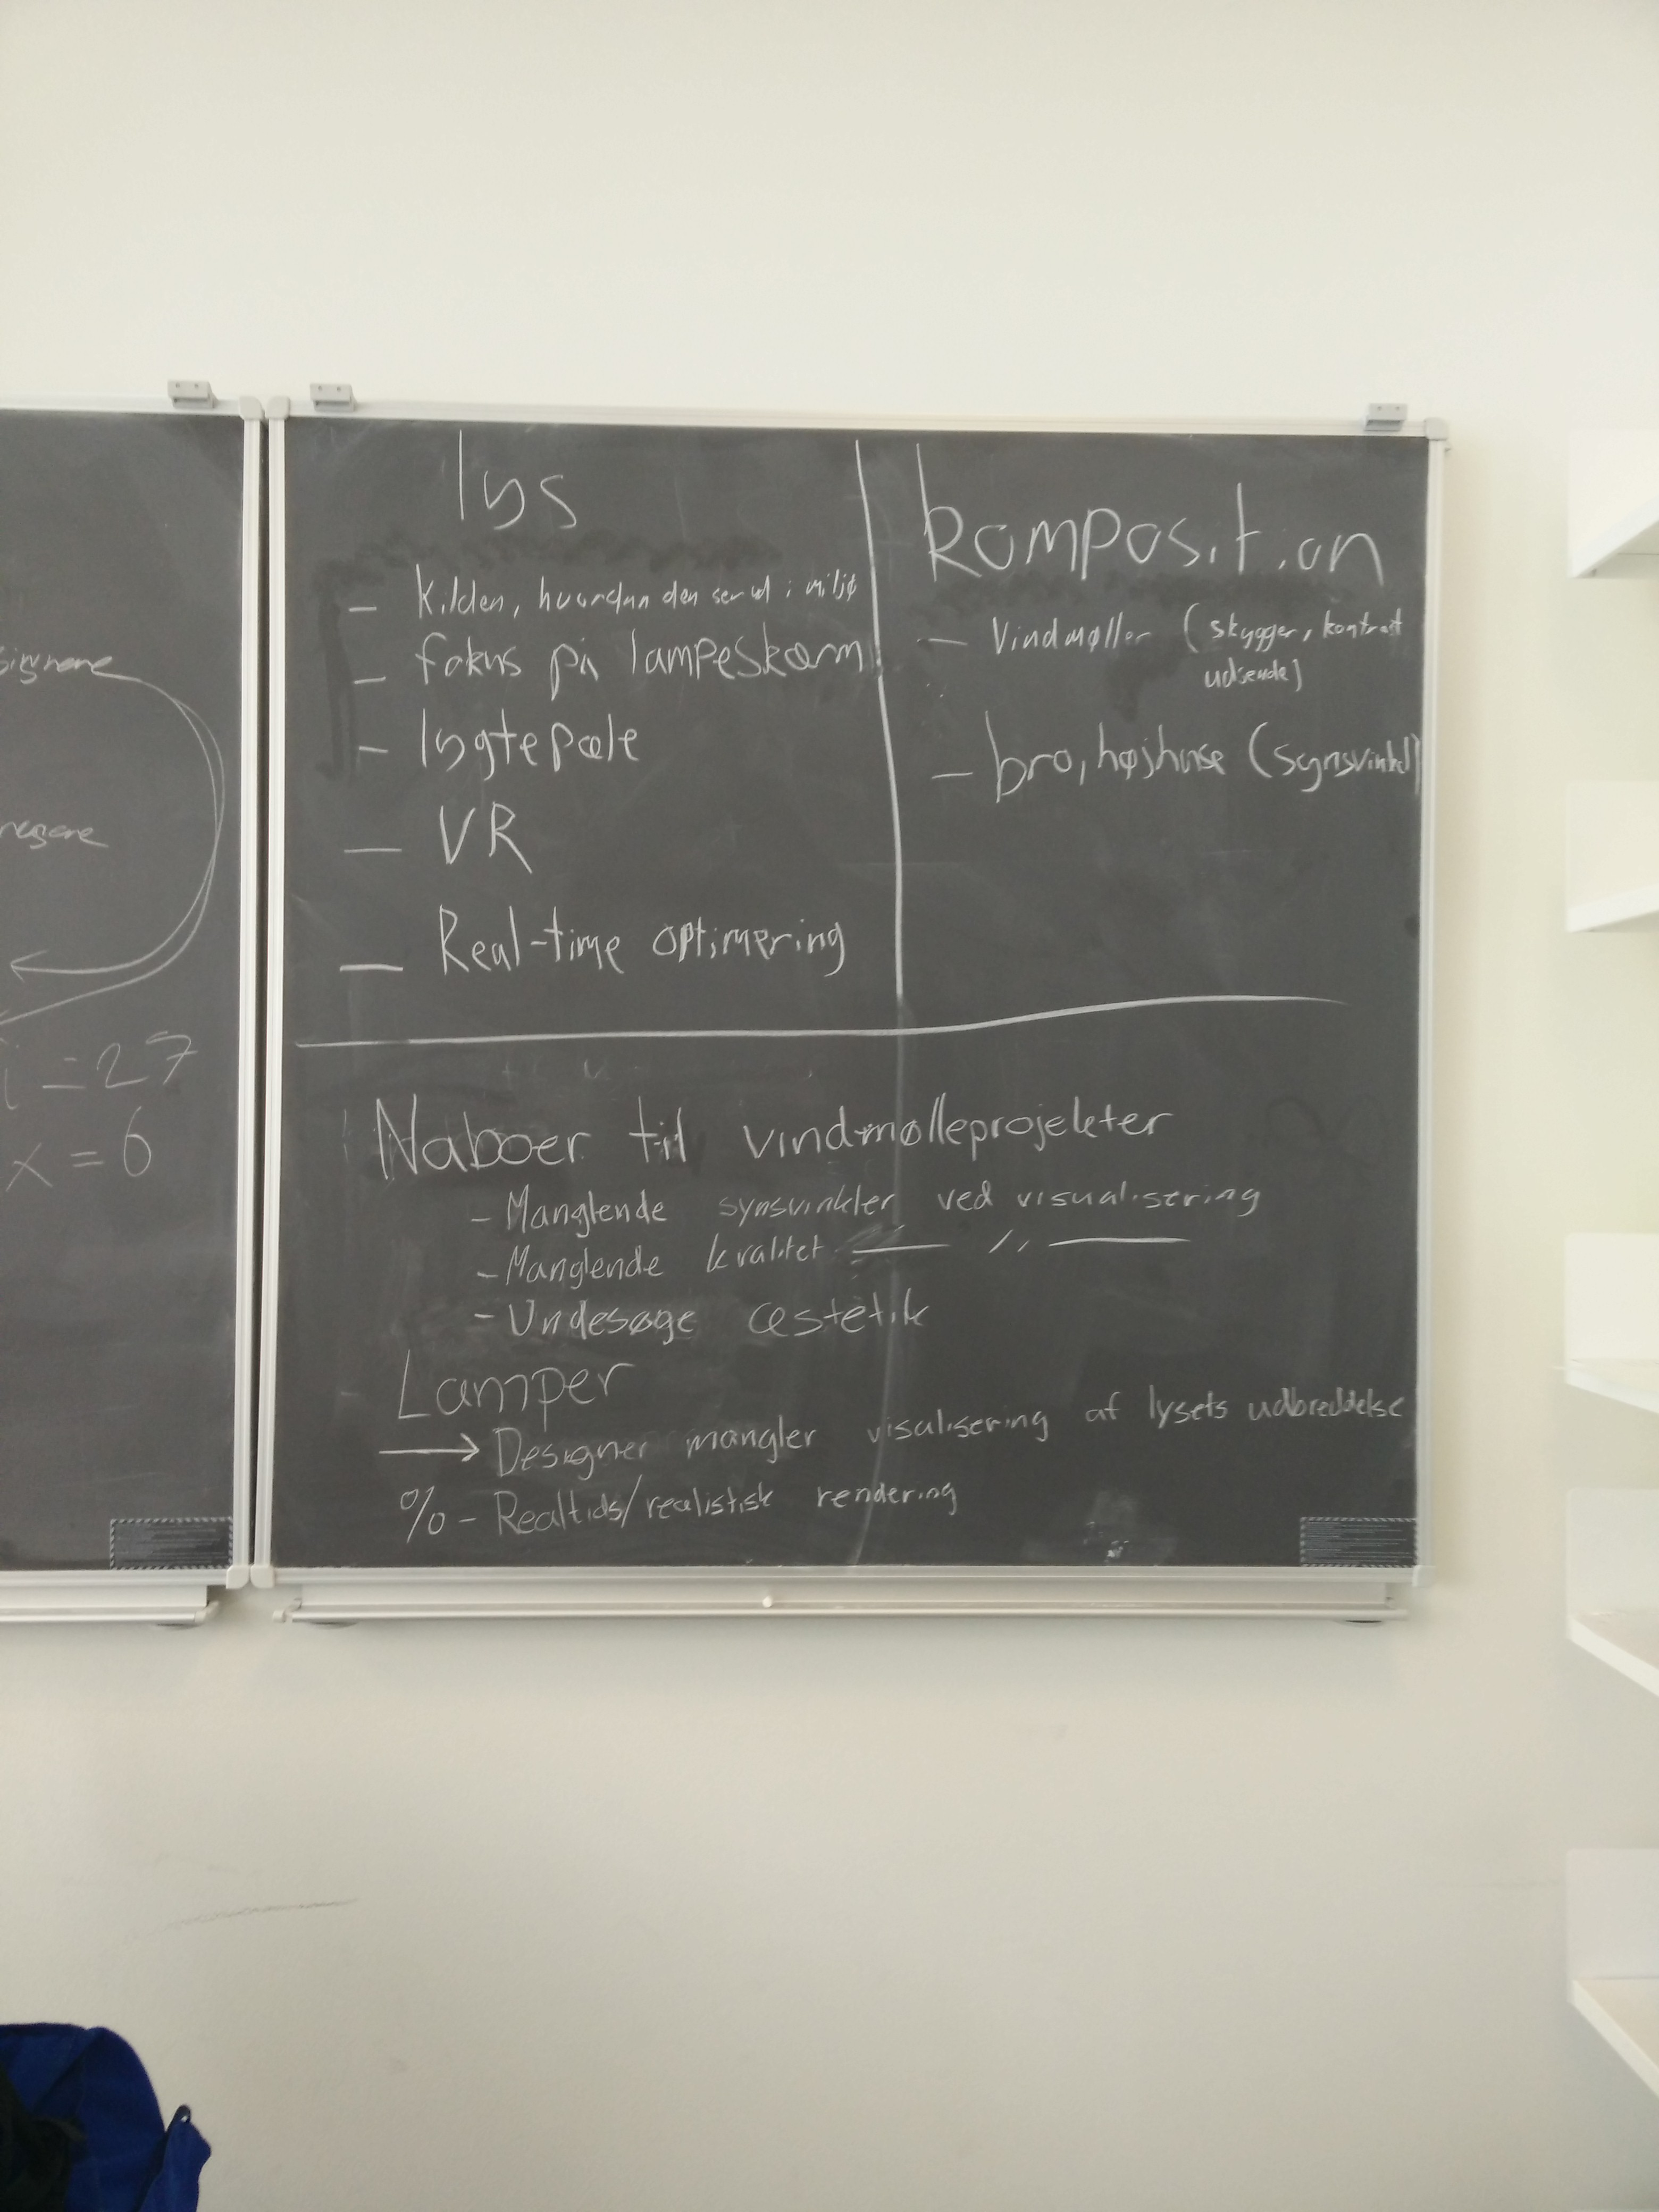
\includegraphics[width=10cm]{./../graphics/brainstorm_1}
   \caption{Billede af første brainstorm}.
\end{figure}

\subsection{Dagsorden}
\begin{figure}[H]
   \centering
   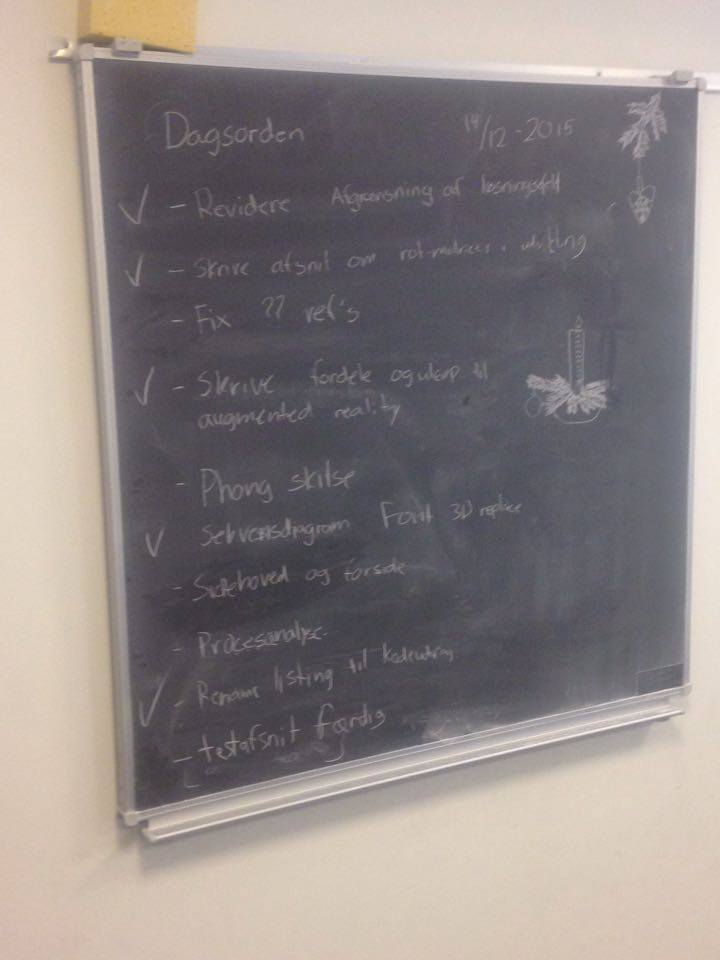
\includegraphics[width=10cm]{./../graphics/dagsorden}
   \caption{Billede af en god dagsorden}.
   \label{fig:dagsorden}
\end{figure}

\end{document}
